\documentclass[main.tex]{subfiles}
\begin{document}
\chapter{Conclusion and Future Work}
\label{chap:concl}
\textbf{\textcolor{red}{fahrplan: mehr oder weniger chapter-wise summary}}

% \paragraph{intro summary}
% \begin{itemize}
%     \item modern man-made environments contain a large number of planar structures, especially indoors
%     \item automatic plane detection has become a vital part of many applications and systems   
%     \item if a time constraint for the calculations exist, it is often referred to as real-time 
%     \item real-time plane detection does exist. However, the sensors that enable real-time plane detection are usually not affordable for the general user
%     \item In this thesis, we compared a selection of plane detection algorithms to evaluate the extents of real-time plane detection on affordable hardware like intel realsense 
% \end{itemize}
\textbf{\textcolor{red}{da intro noch nicht steht werden sich teile hiervon noch ändern müssen}}
Modern man-made environments, especially indoors, contain a large number of planar structures. The automatic detection thereof has become a vital part of many Augmented or Virtual Reality systems. Underlying temporal constraints often dictate the processing times of these applications and, therein, the process of plane detection. \textit{Real-time plane detection} is already possible, although the hardware cost that enables efficient and precise detection is likely not affordable to the general consumer.
Therefore, the extent of \textit{real-time plane detection} on affordable hardware has gained interest.

% \paragraph{concept summary}
% \begin{itemize}
%     \item A set of algorithms, appropriate datasets, and a definition of real-time are needed to perform this evaluation.
%     \item in subsection X we introduced relevant criteria for the selection of algorithms.
%     \item Based on these criteria, we filtered the current state of the art and stuck with four algorithms, namely XY
%     \item We proceeded to select suitable datasets for our evaluation, starting with a set of requirements. 
%     \item We selected the 2D-3D-S dataset and, because our research did not yield a sufficient incrementally growing dataset with plane-focused ground truth, we created the FIN dataset
%     \item Closing Chapter 3, we gave two definitions of realtime
% \end{itemize}

A set of plane detection algorithms, appropriate datasets, and a definition of \textit{real-time} are needed to perform this evaluation. In the \textit{Concept}, we first introduced a set of helpful criteria for the subsequent selection of plane detection algorithms. We followed the same approach for the selection of datasets. Lastly, we introduced two definitions of \textit{real-time}, wherein we differentiate between \textit{real-time} calculation time with and without pre-processing.

% \paragraph{impl summary}
% \begin{itemize}
%     \item we gave details regarding the implementation processes and requirements therein
%     \item Moreover, since the ground truth of the datasets needed modification, we manually segmented planes, which is outlined as well in chapter~4
% \end{itemize}
In Chapter~\ref{chap:impl}, we provided details regarding the implementation of the selected algorithms. Moreover, since its provided ground truth does not focus on planes, we described our manual segmentation process of the 2D-3D-S dataset. Lastly, we outlined how the ground truth for the FIN dataset is dynamically created based on a single ground truth of the last recorded point cloud.

% \paragraph{evaluation summary}
% \begin{itemize}
%     \item We started the evaluation with the protocol. therin, we give the metrics the eval is based on.
%     \item additionally, we specify the parameterizations each algorithm used for the different experiments  
%     \item we presented the individual results and compared the experiments
% \end{itemize}
We enter Chapter~\ref{chap:eval} with the evaluation protocol. Therein, we outline the evaluation metrics to calculate and specify the algorithm parameterizations of each experiment. We presented the individual results and subsequently concluded with a comparison thereof.

% results
% \begin{itemize}
%     \item Without additional modifications, 3D-KHT is the fastest out of the algorithms, on average 32x faster total times
%     \item Nonetheless, RSPD has the overall highest accuracy with ca 87\% in the 2D-3D-S and 58\% in the FIN exp. (F1)
%     \item RPSD has the overall longest pre-processing time, taking on avg 63 and 15 seconds for the normal estimation
%     \item OPS has the overall highest precision, OBRG overcomes no other algorithm in a metric. 
% \end{itemize}

% accuracy
In both experiments, RSPD has the overall best accuracy among the algorithms. While OPS and OBRG achieve a similar average \textit{Precision}, no other algorithm yields comparable values for \textit{Recall} nor \textit{F1-Score} (see Tables~\ref{tab:res-3d2ds-total} and \ref{tab:res-fin-total}). The accuracy metrics of all algorithms drop by roughly $30\%$ from the \textit{2D-3D-S} experiment to the \textit{FIN} experiment.

% times
The results uniformly show that 3D-KHT is the fastest among the selected algorithms. The \textit{Hough Transform}-based algorithm proposed by \citeauthor{LimbergerOliveira2015HT3D}~\cite{LimbergerOliveira2015HT3D} ran, on average, 32x faster as the other algorithms. As Table~\ref{tab:algo-rt} indicates, 3D-KHT is the only algorithm that achieves $RT_{tot}$ in the \textit{FIN} experiment, which is supported by the apparent upper limit shown in Figure~\ref{fig:dynaudi}. RSPD achieves $RT_{calc}$, and OPS borders on \textit{real-time plane detection} as well. RSPD has the longest pre-processing times with an average of ${\sim}63s$ for the \textit{2D-3D-S} experiment and ${\sim}15s$ for the \textit{FIN} experiment, respectively. In contrast, RSPD has the shortest average plane detection times in the \textit{FIN} experiment, and takes only a tenth of a second longer than 3D-KHT's plane detection phase in the \textit{2D-3D-S} experiment.

% Summary 
We can conclude that 3D-KHT is the only algorithm that is \textit{totally real-time} applicable. However, considering accuracy, 3D-KHT is inferior to RSPD.


\section{Limitations}
\textbf{\textcolor{red}{fahrplan: je ein paragraph pro sache die mir einfällt, die die ergebnisse eingeschränken könnte}}
This section deals with the limitations of the concept, evaluation, and results thereof.
% \begin{itemize}
%     \item da fokus der arbeit nicht auf der optimierung von algorithmen lag, sind die parameter wahrscheinlich nicht die 100\% besten für die datensätze
%     \item wie schon \textbf{\textcolor{purple}{irgendwo }}gesagt, ist die manuelle segmentierung sehr subjektiv
%     \item keine maß für die relevanz von ebenen. ein monitor ist erstmal genauso "wichtig" wie eine Wand. (\textbf{\textcolor{red}{useful?}})
%     \item \textbf{\textcolor{red}{dynamische generierung ist nicht perfekt, wenn die sensor daten eine größere streuung haben als die voxel gross sind}}
% \end{itemize}
\paragraph{Algorithm Parameterization}
Since the focus of this work is not the optimization of plane detection algorithms but rather the evaluation thereof, the parameterizations used during the experiments are likely non-optimal. Furthermore, the required effort would go beyond the scope of this work. Integrating a plane detection algorithm into an application would require extensive parameter optimization w.r.t. the expected environment, the used sensors, and the general use case.

\paragraph{Manual Segmentation}
Another limitation of the results is the subjective nature of the manual segmentation process described in Section~\ref{sec:gtseg}, which influences the evaluation. The effect thereof does not seem significant for the \textit{2D-3D-S} experiment. However, the segmentation can lead to errors due to the level of noise in the \textit{FIN} dataset. For instance, with increasing "thickness" of planes, the number of possible orientations of a detected plane also increases (see Figure~\ref{fig:poss-planes}). The red segment in the figure represents the ground truth we selected to represent the plane. If an algorithm detected a plane in one of the four other variants, both the voxel overlap and the accuracy would decrease, even if both planes correspond.

\paragraph{Used Technology}
A small caveat to note is that the FIN dataset is recorded using a specific combination of technology, namely Intel's T265, D455, and the corresponding SDK including RTAB-MAP.
\textbf{\textcolor{red}{unsere ergebnisse zeigen den besten algo für den spezifischen use case, dass jemand ohne großen zeitdruck durch die uni schlendert. würde zb ein spiel hastige bewegungen voraussetzen, würden die aufnahmen anders aussehen und somit möglicherweise andere ergebnisse produzieren.}}

\begin{figure}
    \centering
    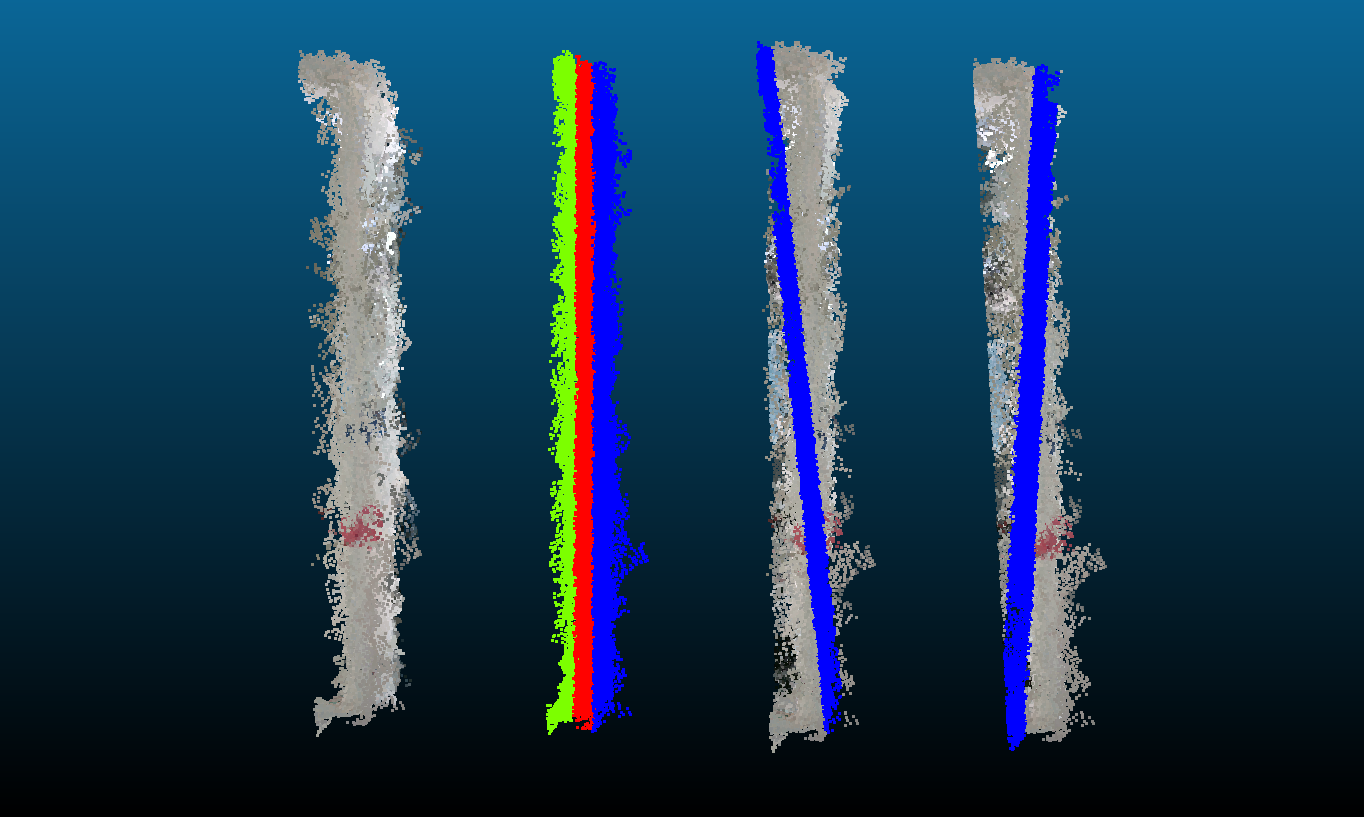
\includegraphics[width=0.7\textwidth]{images/possible_planes.png}
    \caption[Plane Orientation Ambiguity]{Possible Plane Orientations. A wall with a width of ${\sim}1$m from the \textit{conference room} scene of the \textit{FIN} dataset is shown on the left. The colored point clouds indicate different possible plane orientations.}
    \label{fig:poss-planes}
\end{figure}

\section{Future Work}
\textbf{\textcolor{red}{fahrplan: je ein paragraph pro sache die mich jetzt interessieren würde anhand der gewonnenen kenntnisse}}
% \begin{itemize}
%     \item some sensors or SLAM algorithms (including Intels/RTABMAP) are capable of exporting normal vectors. The algorithms would not need to estimate them during their pre-processing phase. 
%     \item OPS and OBRG would benefit as well see Table~\ref{tab:pre-post}
%     \item however the extents of this improvement are up for future work.
%     \item For RSPD, this would essentially reduce the pre-processing times to a minimum and with it, the total processing time as well. We consider this the most promising endeavor. however this would of course require the normal exportation from sensor, or SLAM. intel kann das, wäre also nicht zwangsweise mit extra kosten verbunden.
% \end{itemize}

\paragraph{Normal Estimation}
We see the most potential for improvement in the pre-processing steps of the algorithms. Specifically, the extent of the normal vector estimation influences the pre-processing time. RSPD estimates the normal vectors of the entire point cloud, whereas OPS only estimates $\alpha_s$\% of the point cloud. This temporal difference raises the question of what the extents of \textit{real-time plane detection} are if the normal vectors of the point cloud are known before the plane detection step in the application. For instance, RTAB-MAP can estimate and export the normal vectors of the point cloud. Therefore, RSPD would not need to estimate the normal vectors, reducing the pre-processing time greatly. However, this would require further research.

\paragraph{Cloud Size Reduction}
When recording environments similar to the hallway or the auditorium scene, it is often the case that the spatial dimension of the point cloud grows beyond the distance limitations of the sensor, e.g., the recorded hallway spans longer than the sensor can "see". It is, therefore, not necessary to re-calculate the planes in areas past the sensor's reach. We are interested in a plane detection method that restricts the plane detection to a certain radius around the sensor's position and a subsequent merging of old and new planes. Additionally, this could be the basis for a plane-based SLAM approach.

\paragraph{Outdoor Environment}
In Chapter~\ref{chap:Introduction}, we limited ourselves to evaluating plane detection algorithms in indoor environments. Therefore, we cannot make any statements about the applicability in outdoor environments. Since we compiled results in a realistic indoor environment, it would be interesting to evaluate the generalization of these algorithms. As discussed throughout this thesis, a comparison needs uniformity. Since we created an indoor dataset, selected datasets, and provided all necessary metrics and definitions, only an appropriate dataset is needed.

% \begin{itemize}
%     \item C++ impl von OBRG
%     \item reduzierung der plane detection auf 6m circumference und merging danach
%     \item normal export durch SLAM, experimente wiederholen
%     \item \textbf{\textcolor{red}{dynamische generierung verbessern? $\rightarrow$ }}
% \end{itemize}

\end{document}